\begin{figure}[!b]
\centering
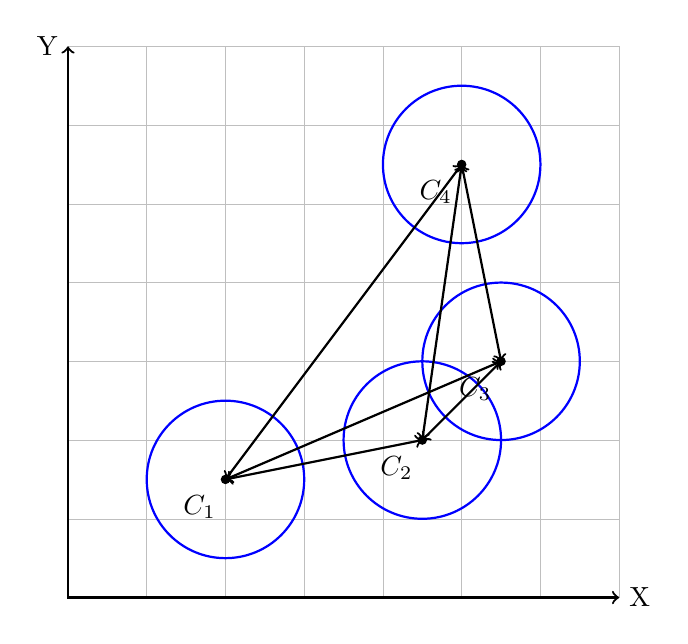
\begin{tikzpicture}[scale=1]
% grid
    \draw[very thin,color=lightgray] (0,0) grid (7,7);
    \draw [<->,thick] (0,7) node (yaxis) [left] {Y} |- (7,0) node (xaxis) [right] {X};
    
    %Index, x, y, r
    \def\circle[#1,#2,#3,#4] {
    	%The middlepoint
    	\coordinate (C#1) at (#2,#3);
    	
    	%The point
		\draw[fill,color=black] (C#1) circle (1.5pt) node[left, yshift=-10pt, color=black] {$C_#1$};
		
		%The circle
		\draw[thick,color=blue] (C#1) circle (#4);

	}
	
	\circle[1,2,1.5,1]
	\circle[2,4.5,2,1]    
    \circle[3,5.5,3,1]
    \circle[4,5,5.5,1]
    

	\draw[thick,<->] (C1) -- (C2);
	\draw[thick,<->] (C1) -- (C3);
	\draw[thick,<->] (C1) -- (C4);
	\draw[thick,<->] (C2) -- (C3);
	\draw[thick,<->] (C2) -- (C4);
	\draw[thick,<->] (C3) -- (C4);

       
\end{tikzpicture}
\label{fig:voorbeeld_1}
\end{figure}